\subsection{矩阵轨迹}
训练前在独立种子101上比较各候选的峰值学习率，选择500步后的最小目标值。
正式种子0至9共享初始目标值1，匹配优化器使用的随机噪声序列。
每10步记录真梯度范数与目标值。图\ref{fig:v2trajectory}按种子计算均值和样本标准差。

\begin{figure}[htbp]\centering
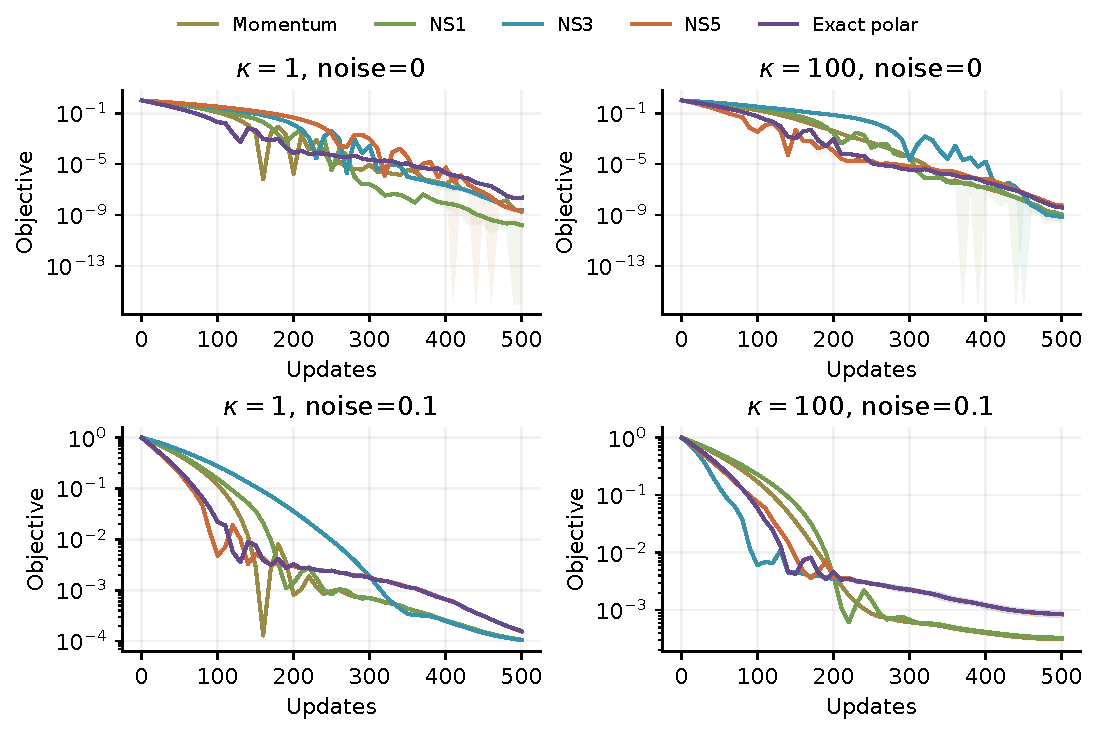
\includegraphics[width=\linewidth]{figures_v2/v2_matrix_trajectories.pdf}
\caption{倒置曲率的矩阵优化轨迹。横轴为更新步数，纵轴为目标值，阴影为10个种子的一个样本标准差。}
\label{fig:v2trajectory}
\end{figure}

\subsection{验证、测试与冻结更新}
WikiText103的验证集与测试集分别有251048和287644个预测目标。
TinyStories的验证使用固定的262144个目标，测试共2369481个目标。
数据按连续token分块，尾块只累计实际目标。
种子配对使用完整的同一训练步数。测试分数取该种子在验证损失最低点保存的模型。

在主实验的NS5与Probe-NS、较大模型的NS5、TinyStories的NS5四组中，
每种子保存3个更新前状态，共36个锚点。
每个锚点保存基础参数、训练动量、候选全量更新和数据身份。
从实际存档步长中扣除权重衰减后，隐藏矩阵方向RMS与目标0.2的最大差为$4.59\times 10^{-8}$。
谱统计使用首层融合QKV、中层MLP上投影、末层注意力输出和MLP下投影四个矩阵。
局部曲率和完整步长响应使用float32计算。

\begin{figure}[htbp]\centering
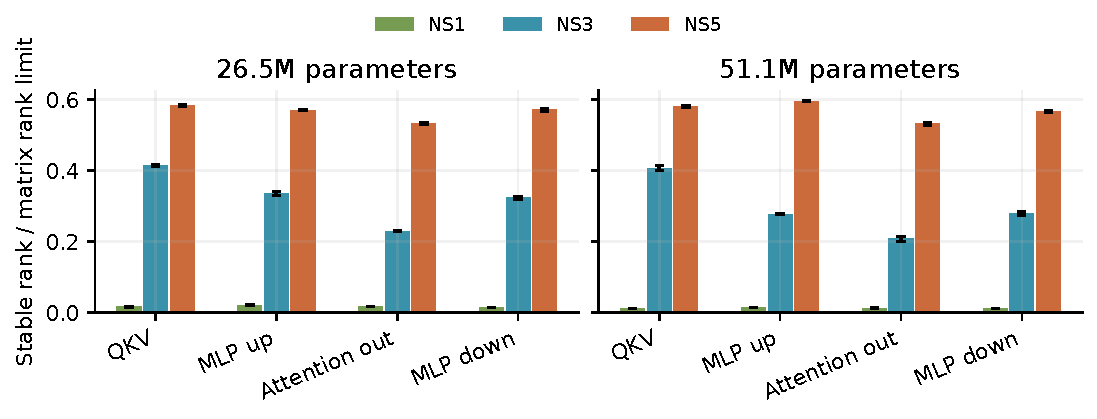
\includegraphics[width=\linewidth]{figures_v2/v2_update_spectra.pdf}
\caption{WikiText103中实际候选更新的谱形状。稳定秩除以矩阵的最大可能秩。
每个种子内先在锚点上平均，误差条为三个种子的样本标准差。}
\label{fig:v2spectra}
\end{figure}

\subsection{重放深度与实际干预长度}
表\ref{tab:v2replay}给出每个种子的探测选择与重放序列。
第100、200、\ldots、1000步发生选择。末次选择只作用于第1000步，重放固定该位置。
表的最后一列把不同的选择换算成实际采用不同深度的更新数。
\begin{table}[htbp]\centering
\caption{目标反馈和阶段匹配重放的逐种子选择。}
\label{tab:v2replay}
\begin{tabular}{cllr}
\toprule
种子 & Probe-NS深度 & 重放深度 & 改动步数 \\ \midrule
0 & 5,5,5,5,5,5,5,5,5,5 & 5,5,5,5,5,5,5,5,5,5 & 0 \\
1 & 5,5,5,5,5,5,5,5,3,5 & 5,5,5,5,5,5,5,5,3,5 & 0 \\
2 & 5,5,5,5,5,5,5,5,3,5 & 5,5,5,5,5,5,5,5,3,5 & 0 \\
\bottomrule
\end{tabular}

\end{table}
